\documentclass[border=1pt]{standalone}
% ---------------------------------------------------------------------------
% Shared style for the MOSAIC / CRYSTAL TOMM figures.
% Compile each fig_*.tex with LuaLaTeX (standalone). Sized for acmart
% "acmsmall" (TOMM): \textwidth = 13.9 cm, so every figure is drawn at
% final size and is included with width=\textwidth (no rescaling of text).
% Fonts: Libertinus Sans + Inconsolata (acmart uses Libertine + Inconsolata).
% ---------------------------------------------------------------------------
\usepackage{fontspec}
\setmainfont{LibertinusSans}[Path=fonts/, Extension=.otf,
  UprightFont=*-Regular, BoldFont=*-Bold, ItalicFont=*-Italic]
\setmonofont{Inconsolata}[Path=fonts/, Extension=.otf,
  UprightFont=*-Regular, BoldFont=*-Bold, Scale=0.98]
\usepackage{unicode-math}
\setmathfont{LibertinusMath-Regular.otf}[Path=fonts/]

\usepackage{tikz}
\usetikzlibrary{positioning,fit,calc,arrows.meta,backgrounds,
  shapes.misc,shapes.geometric,decorations.pathreplacing,patterns.meta}

% Okabe-Ito palette (colour-blind safe) + tints -------------------------------
\definecolor{oiBlue}{HTML}{0072B2}
\definecolor{oiOrange}{HTML}{E69F00}
\definecolor{oiSky}{HTML}{56B4E9}
\definecolor{oiGreen}{HTML}{009E73}
\definecolor{oiVerm}{HTML}{D55E00}
\definecolor{oiPurple}{HTML}{CC79A7}
\definecolor{oiYellow}{HTML}{F0E442}
\definecolor{ink}{HTML}{1A1A1A}
\definecolor{muted}{HTML}{5C5C5C}
\definecolor{rule}{HTML}{9A9A9A}

\definecolor{oursFill}{HTML}{DDEBF7}
\definecolor{oursDraw}{HTML}{0072B2}
\definecolor{modFill}{HTML}{FCEFD2}
\definecolor{modDraw}{HTML}{B57600}
\definecolor{upFill}{HTML}{F1F1F1}
\definecolor{upDraw}{HTML}{7D7D7D}
\definecolor{failFill}{HTML}{FBE3D6}
\definecolor{okFill}{HTML}{D9F0E8}

% Sequence colours (as in the packetization study)
\definecolor{seqSOL}{HTML}{0072B2}
\definecolor{seqTHA}{HTML}{009E73}
\definecolor{seqLON}{HTML}{CC79A7}

% Typography -----------------------------------------------------------------
\newcommand{\figfont}{\fontsize{7.5}{9}\selectfont}
\newcommand{\smallfig}{\fontsize{6.5}{7.8}\selectfont}
\newcommand{\tinyfig}{\fontsize{6}{7.2}\selectfont}
\newcommand{\code}[1]{{\ttfamily #1}}

% Provenance encoding: colour AND line style (grayscale safe) ------------------
%  ours      = new component written by us      (blue, solid 0.9 pt)
%  modified  = upstream component we patched    (orange, dashed 0.8 pt)
%  upstream  = used unmodified / third party    (grey, solid 0.45 pt)
\tikzset{
  base/.style={rectangle, rounded corners=1.6pt, align=center,
    inner xsep=3pt, inner ysep=2.6pt, font=\figfont, text=ink,
    execute at begin node={\hyphenpenalty=10000\exhyphenpenalty=10000}},
  ours/.style={base, fill=oursFill, draw=oursDraw, line width=0.9pt},
  mod/.style={base, fill=modFill, draw=modDraw, line width=0.8pt,
    dash pattern=on 2.6pt off 1.4pt},
  up/.style={base, fill=upFill, draw=upDraw, line width=0.45pt},
  dead/.style={base, fill=white, draw=oiVerm, line width=0.6pt,
    dash pattern=on 1.2pt off 1.2pt, text=oiVerm},
  note/.style={font=\smallfig, text=muted, align=left,
    execute at begin node={\hyphenpenalty=10000\exhyphenpenalty=10000}},
  lab/.style={font=\smallfig\itshape, text=muted},
  zone/.style={draw=rule, line width=0.45pt, rounded corners=3pt,
    dash pattern=on 0.6pt off 1.1pt},
  zonetitle/.style={font=\figfont\bfseries, text=ink, anchor=west,
    inner xsep=2pt, inner ysep=1pt, fill=white, xshift=2.5mm},
  flow/.style={-{Stealth[length=4pt,width=3.2pt]}, line width=0.65pt,
    draw=ink},
  dflow/.style={flow, dash pattern=on 2pt off 1.4pt},
  ctrl/.style={-{Stealth[length=3.4pt,width=2.8pt]}, line width=0.5pt,
    draw=muted},
  failflow/.style={-{Stealth[length=4pt,width=3.2pt]}, line width=0.6pt,
    draw=oiVerm, dash pattern=on 1.4pt off 1.2pt},
  stepc/.style={circle, fill=ink, text=white, inner sep=0pt,
    minimum size=8.5pt, font=\tinyfig\bfseries},
  tag/.style={font=\tinyfig\bfseries, inner sep=1pt},
}

% Legend for the provenance encoding -------------------------------------------
\newcommand{\provlegend}[1]{% #1 = anchor coordinate (north west)
  \begin{scope}[shift={(#1)}]
    \node[ours, minimum width=6mm, minimum height=2.6mm, inner sep=0pt]
      (lg1) at (0,0) {};
    \node[anchor=west, font=\smallfig] at (lg1.east) {new (this work)};
    \node[mod, minimum width=6mm, minimum height=2.6mm, inner sep=0pt]
      (lg2) at (2.6,0) {};
    \node[anchor=west, font=\smallfig] at (lg2.east) {upstream, patched by us};
    \node[up, minimum width=6mm, minimum height=2.6mm, inner sep=0pt]
      (lg3) at (6.2,0) {};
    \node[anchor=west, font=\smallfig] at (lg3.east) {upstream / third party, unmodified};
  \end{scope}}

\newcommand{\bx}[2]{{\bfseries #1\par}\vspace{0.6pt}{\smallfig #2\par}}
\begin{document}
\figfont
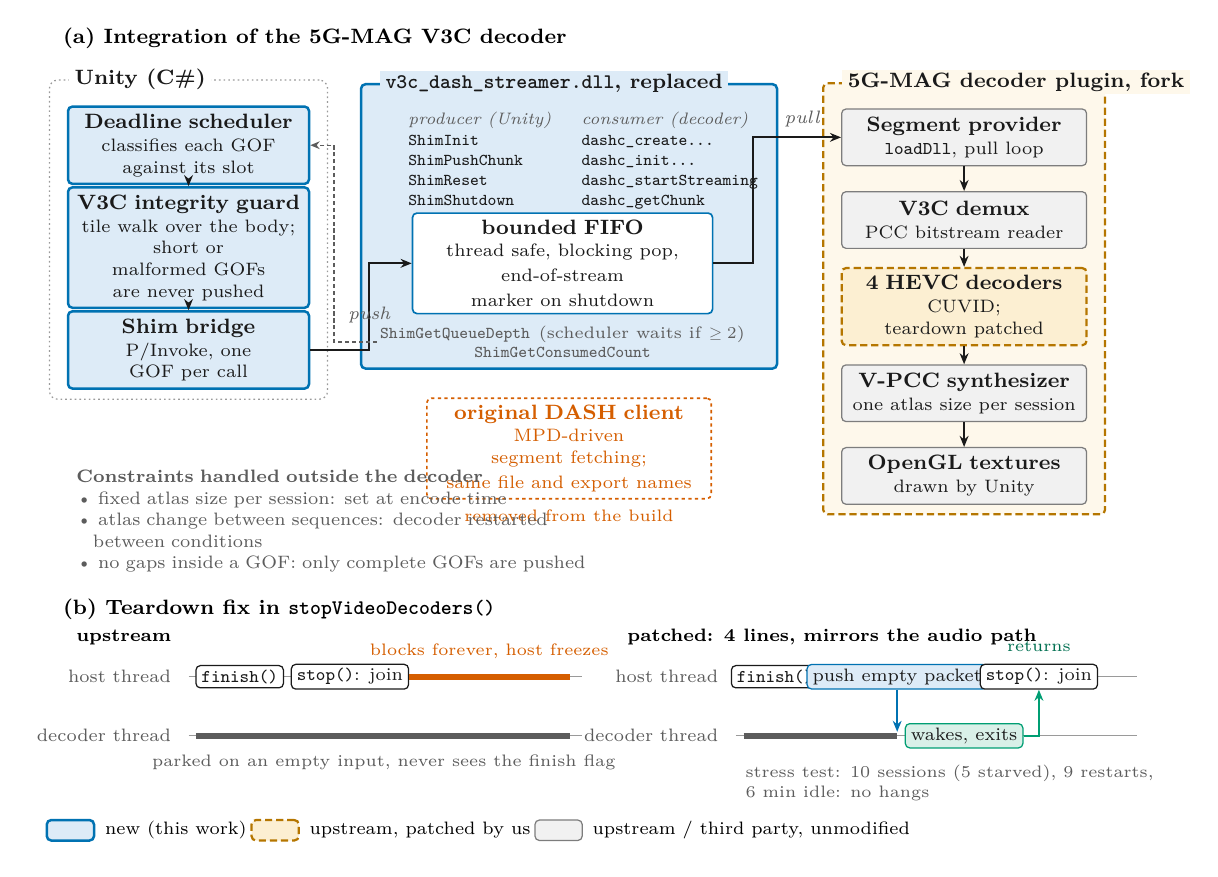
\begin{tikzpicture}[x=1cm,y=1cm]
  \tikzset{w/.style={text width=2.85cm, minimum height=0.9cm},
           api/.style={font=\tinyfig\ttfamily, text=ink, align=left, inner sep=1pt},
           apih/.style={font=\tinyfig\itshape, text=muted, align=left, inner sep=1pt},
           panel/.style={font=\figfont\bfseries, anchor=north west, inner sep=0pt}}

  \node[panel] at (0,9.45) {(a) Integration of the 5G-MAG V3C decoder};

  % ------------------------------ Unity side --------------------------------
  \node[ours, w] (sch) at (1.6,7.95) {\bx{Deadline scheduler}{classifies each GOF\\against its slot}};
  \node[ours, w] (grd) at (1.6,6.65) {\bx{V3C integrity guard}{tile walk over the body;\\short or malformed GOFs\\are never pushed}};
  \node[ours, w] (brg) at (1.6,5.35) {\bx{Shim bridge}{P/Invoke, one GOF per call}};
  \draw[flow] (sch) -- (grd);
  \draw[flow] (grd) -- (brg);
  \begin{scope}[on background layer]
    \node[zone, fit=(sch)(grd)(brg), inner sep=2.2mm, yshift=1mm] (zu) {};
  \end{scope}
  \node[zonetitle] at (zu.north west) {Unity (C\#)};

  % ------------------------------ push-queue shim ----------------------------
  \node[base, draw=oursDraw, fill=white, line width=0.6pt, text width=3.6cm,
        minimum height=1.05cm] (fifo) at (6.35,6.45)
     {{\bfseries bounded FIFO}\par{\smallfig thread safe, blocking pop,\\end-of-stream marker on shutdown}};
  \node[apih, anchor=south west] (ph) at (4.35,8.12) {producer (Unity)};
  \node[api, anchor=north west] (pin) at (ph.south west) {ShimInit\\ShimPushChunk\\ShimReset\\ShimShutdown};
  \node[apih, anchor=south west] (ch) at (6.55,8.12) {consumer (decoder)};
  \node[api, anchor=north west] (pout) at (ch.south west) {dashc\_create...\\dashc\_init...\\dashc\_startStreaming\\dashc\_getChunk};
  \node[api, anchor=north, text=muted, align=center] (ptel) at ($(fifo.south)+(0,-0.1)$)
     {ShimGetQueueDepth \textrm{(scheduler waits if} $\geq 2$\textrm{)}\\ShimGetConsumedCount};
  \begin{scope}[on background layer]
    \node[ours, fit=(ph)(ch)(pin)(pout)(fifo)(ptel), inner sep=2.0mm, yshift=1.1mm] (zs) {};
  \end{scope}
  \node[zonetitle, fill=oursFill] at (zs.north west) {\code{v3c\_dash\_streamer.dll}, replaced};
  \node[dead, text width=3.4cm, anchor=north] (orig) at ($(zs.south)+(0,-0.35)$)
     {{\bfseries original DASH client}\par{\smallfig MPD-driven segment fetching;\\same file and export names}};
  \node[font=\tinyfig, text=oiVerm, anchor=north] at (orig.south) {removed from the build};

  \draw[flow] (brg.east) -- ++(0.75,0) |- (fifo.west) node[pos=0.1, above, lab] {push};
  \draw[ctrl, dash pattern=on 1.5pt off 1pt] (ptel.west) -| ($(sch.east)+(0.3,0)$) -- (sch.east);
  

  % ------------------------------ decoder plugin (patched) -------------------
  \tikzset{dw/.style={up, text width=2.9cm, minimum height=0.72cm}}
  \node[dw] (ld)  at (11.45,8.05) {\bx{Segment provider}{\code{loadDll}, pull loop}};
  \node[dw] (dmx) at (11.45,7.0) {\bx{V3C demux}{PCC bitstream reader}};
  \node[mod, text width=2.9cm, minimum height=0.72cm] (vd) at (11.45,5.9)
     {\bx{4 HEVC decoders}{CUVID; teardown patched}};
  \node[dw] (syn) at (11.45,4.8) {\bx{V-PCC synthesizer}{one atlas size per session}};
  \node[dw] (gl)  at (11.45,3.75) {\bx{OpenGL textures}{drawn by Unity}};
  \draw[flow] (ld) -- (dmx); \draw[flow] (dmx) -- (vd);
  \draw[flow] (vd) -- (syn); \draw[flow] (syn) -- (gl);
  \begin{scope}[on background layer]
    \node[mod, fit=(ld)(dmx)(vd)(syn)(gl), inner sep=2.2mm, yshift=1mm, fill=modFill!45] (zd) {};
  \end{scope}
  \node[zonetitle, fill=modFill!45] at (zd.north west) {5G-MAG decoder plugin, fork};
  \draw[flow] (fifo.east) -- ++(0.5,0) |- (ld.west) node[pos=0.78, above, lab] {pull};

  % constraints handled outside the decoder
  \node[note, text width=6.6cm, anchor=north west] at (0.05,3.95)
    {\textbf{Constraints handled outside the decoder}\\
     \textbullet\ fixed atlas size per session: set at encode time\\
     \textbullet\ atlas change between sequences: decoder restarted\\\hspace*{6pt}between conditions\\
     \textbullet\ no gaps inside a GOF: only complete GOFs are pushed};

  % ======================== panel (b): teardown fix ===========================
  \node[panel] at (0,2.2) {(b) Teardown fix in \code{stopVideoDecoders()}};
  \tikzset{lane/.style={font=\smallfig, text=muted, anchor=east},
           act/.style={base, font=\smallfig, fill=white, draw=ink, line width=0.45pt,
              inner xsep=2pt, inner ysep=1.5pt},
           wait/.style={draw=muted, line width=2.2pt, line cap=butt}}
  % upstream
  \node[font=\smallfig\bfseries, anchor=west] at (0.05,1.7) {upstream};
  \node[lane] at (1.5,1.2) {host thread};
  \node[lane] at (1.5,0.45) {decoder thread};
  \draw[rule, line width=0.4pt] (1.6,1.2) -- (6.6,1.2);
  \draw[rule, line width=0.4pt] (1.6,0.45) -- (6.6,0.45);
  \node[act] (u1) at (2.25,1.2) {\code{finish()}};
  \node[act] (u2) at (3.65,1.2) {\code{stop()}: join};
  \draw[wait, draw=oiVerm] (4.4,1.2) -- (6.45,1.2);
  \node[font=\tinyfig, text=oiVerm, anchor=south] at (5.42,1.3) {blocks forever, host freezes};
  \draw[wait] (1.7,0.45) -- (6.45,0.45);
  \node[font=\tinyfig, text=muted, anchor=north] at (4.08,0.33) {parked on an empty input, never sees the finish flag};

  % patched
  \node[font=\smallfig\bfseries, anchor=west] at (7.05,1.7) {patched: 4 lines, mirrors the audio path};
  \node[lane] at (8.45,1.2) {host thread};
  \node[lane] at (8.45,0.45) {decoder thread};
  \draw[rule, line width=0.4pt] (8.55,1.2) -- (13.65,1.2);
  \draw[rule, line width=0.4pt] (8.55,0.45) -- (13.65,0.45);
  \node[act] (p1) at (9.05,1.2) {\code{finish()}};
  \node[act, draw=oiBlue, fill=oursFill] (p2) at (10.6,1.2) {push empty packet};
  \node[act] (p3) at (12.4,1.2) {\code{stop()}: join};
  \draw[wait] (8.65,0.45) -- (10.6,0.45);
  \draw[flow, draw=oiBlue] (p2.south) -- (10.6,0.5);
  \node[act, fill=okFill, draw=oiGreen] (p4) at (11.45,0.45) {wakes, exits};
  \draw[flow, draw=oiGreen] (p4.east) -| (p3.south);
  \node[font=\tinyfig, text=oiGreen!70!black, anchor=south] at ($(p3.north)+(0,0.03)$) {returns};
  \node[font=\tinyfig, text=muted, anchor=north west, align=left] at (8.55,0.2)
    {stress test: 10 sessions (5 starved), 9 restarts,\\6 min idle: no hangs};

  \provlegend{0.1,-0.75}
\end{tikzpicture}
\end{document}
